%%%%%%%%%%%%%%%%%%%%%%%%%%%%%%%%%%%%%%%%%
% Ay 190 - WS2
% Written by Chatarin Wong-u-railertkun
%%%%%%%%%%%%%%%%%%%%%%%%%%%%%%%%%%%%%%%%%

%----------------------------------------------------------------------------------------
%	PACKAGES AND OTHER DOCUMENT CONFIGURATIONS
%----------------------------------------------------------------------------------------

\documentclass[11pt,letterpaper]{article}

% Load some basic packages that are useful to have
% and that should be part of any LaTeX installation.
%

\usepackage{graphicx}     % be able to include figures

\usepackage{xcolor}         % get nice colors

% change default font to Palatino (looks nicer!)
\usepackage[latin1]{inputenc}
\usepackage{mathpazo}
\usepackage[T1]{fontenc}

% load some useful math symbols/fonts
\usepackage{latexsym,amsfonts,amsmath,amssymb}
\usepackage{subcaption}

% comfort package to easily set margins
\usepackage[top=1in, bottom=1in, left=1in, right=1in]{geometry}

% control some spacings
%
% spacing after a paragraph
\setlength{\parskip}{.15cm}
% indentation at the top of a new paragraph
\setlength{\parindent}{0.0cm}

\usepackage{courier}


%----------------------------------------------------------------------------------------
%	TITLE
%----------------------------------------------------------------------------------------

\begin{document}

\begin{center}
\Large
Ay190 -- Worksheet 11 - Advection Equation \\    %%%%%% DON'T FORGET TO CHANGE THE WORK SHEET NUMBER
Chatarin (Mee) Wong-u-railertkun\\
Date: \today
\end{center}

\section{Analytical answer}
The analytical answer for the advection equation is a Gaussian with shifted center by vt. I don't know how to save the animation in python and import into LaTeX, so if you run the \texttt{Q1.py}, we can see the Gaussian moves along as time progresses.

\section{Upwind Method}

For upwind method, the stability zone is when $0\leq \alpha \leq 1$. In figure \ref{fig:Stability}, we can see that when alpha is out of the stability condition, the error grows significantly.

\begin{figure}[h!]
	\centering
	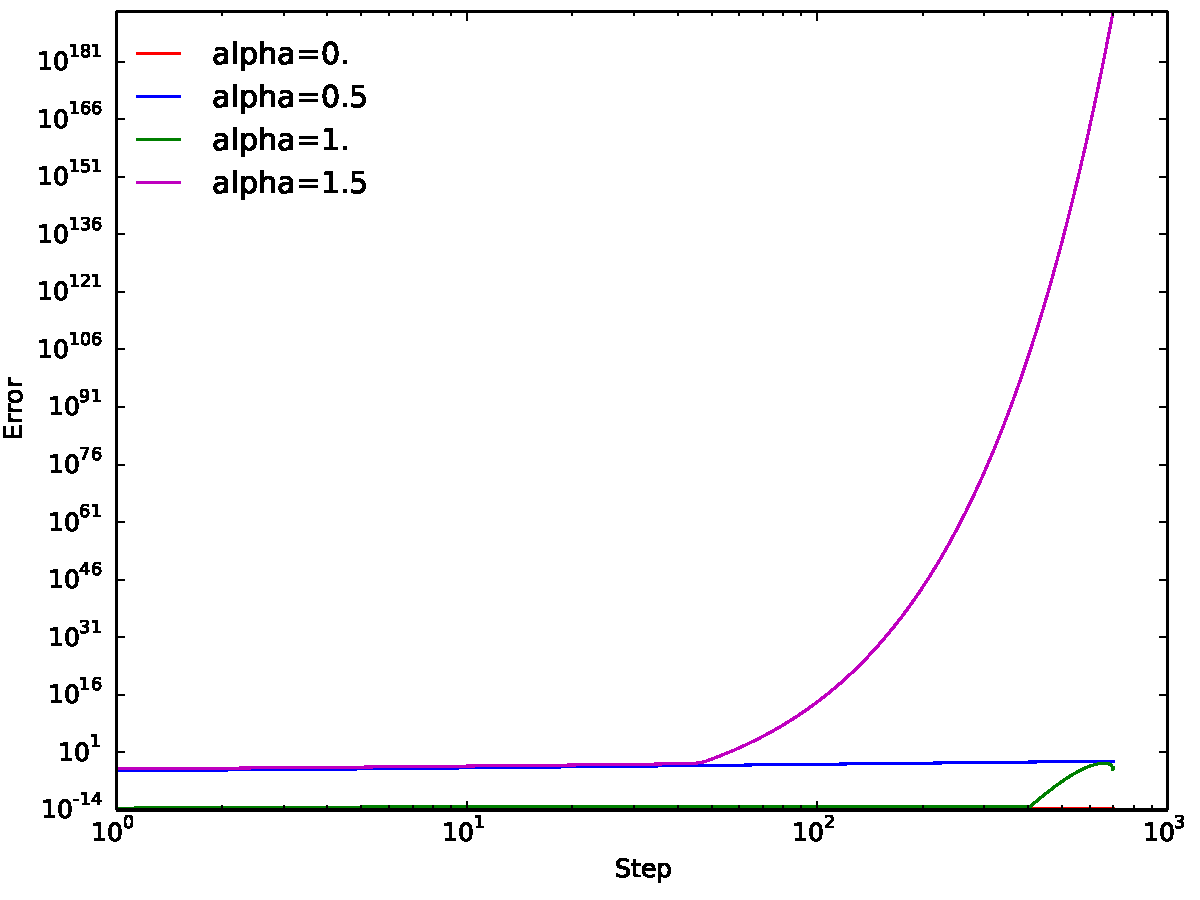
\includegraphics[width=0.5\textwidth]{Stability}
	\caption{The progress of error with different alpha on upwind method.}
	\label{fig:Stability}
\end{figure}

When reduce the initial $\sigma$ by 1/5, when perform the upwind method, as time progress, the peak of Gaussian in numerical upwind method gets smaller and smaller, and the Gaussian gets wider. Run code \texttt{Q2-2.py} to see it.

\section{FTCS Method}

For FTCS Method, it is always unstable. From the visualization, I can see that, start at around iteration 300, the error starts to grow, not at the peak, but before, as packages of sinusoidal beats. (See figure \ref{fig:Stability})

\begin{figure}[h!]
	\centering
	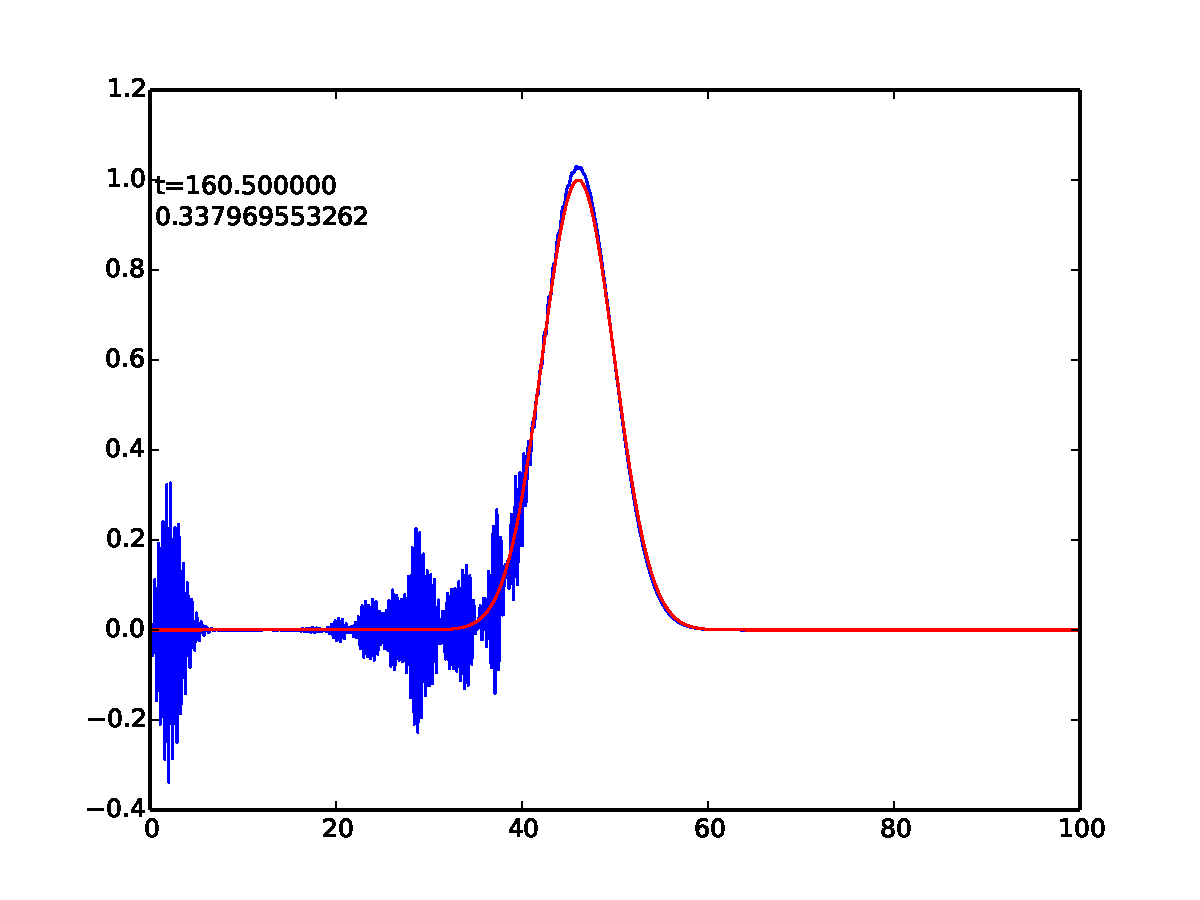
\includegraphics[width=0.5\textwidth]{Instability}
	\caption{Error starts to grow in FTCS method after iteration of 300.}
	\label{fig:Stability}
\end{figure}

\section{Lax-Friedrich Method}
Run \texttt{Q4.py} to visualize. For both upwind and Lax-Friedrich Method, as time progresses, the peak of the Gaussian decreases, but the peak for Lax-Friedrich Method decreases at a faster rate.	
	
\end{document}

